% Options for packages loaded elsewhere
\PassOptionsToPackage{unicode}{hyperref}
\PassOptionsToPackage{hyphens}{url}
\PassOptionsToPackage{dvipsnames,svgnames,x11names}{xcolor}
%
\documentclass[
  letterpaper,
  DIV=11,
  numbers=noendperiod]{scrartcl}

\usepackage{amsmath,amssymb}
\usepackage{iftex}
\ifPDFTeX
  \usepackage[T1]{fontenc}
  \usepackage[utf8]{inputenc}
  \usepackage{textcomp} % provide euro and other symbols
\else % if luatex or xetex
  \usepackage{unicode-math}
  \defaultfontfeatures{Scale=MatchLowercase}
  \defaultfontfeatures[\rmfamily]{Ligatures=TeX,Scale=1}
\fi
\usepackage{lmodern}
\ifPDFTeX\else  
    % xetex/luatex font selection
\fi
% Use upquote if available, for straight quotes in verbatim environments
\IfFileExists{upquote.sty}{\usepackage{upquote}}{}
\IfFileExists{microtype.sty}{% use microtype if available
  \usepackage[]{microtype}
  \UseMicrotypeSet[protrusion]{basicmath} % disable protrusion for tt fonts
}{}
\makeatletter
\@ifundefined{KOMAClassName}{% if non-KOMA class
  \IfFileExists{parskip.sty}{%
    \usepackage{parskip}
  }{% else
    \setlength{\parindent}{0pt}
    \setlength{\parskip}{6pt plus 2pt minus 1pt}}
}{% if KOMA class
  \KOMAoptions{parskip=half}}
\makeatother
\usepackage{xcolor}
\usepackage[top=1in,bottom=1in,left=1in,right=1in,heightrounded]{geometry}
\setlength{\emergencystretch}{3em} % prevent overfull lines
\setcounter{secnumdepth}{-\maxdimen} % remove section numbering
% Make \paragraph and \subparagraph free-standing
\ifx\paragraph\undefined\else
  \let\oldparagraph\paragraph
  \renewcommand{\paragraph}[1]{\oldparagraph{#1}\mbox{}}
\fi
\ifx\subparagraph\undefined\else
  \let\oldsubparagraph\subparagraph
  \renewcommand{\subparagraph}[1]{\oldsubparagraph{#1}\mbox{}}
\fi


\providecommand{\tightlist}{%
  \setlength{\itemsep}{0pt}\setlength{\parskip}{0pt}}\usepackage{longtable,booktabs,array}
\usepackage{calc} % for calculating minipage widths
% Correct order of tables after \paragraph or \subparagraph
\usepackage{etoolbox}
\makeatletter
\patchcmd\longtable{\par}{\if@noskipsec\mbox{}\fi\par}{}{}
\makeatother
% Allow footnotes in longtable head/foot
\IfFileExists{footnotehyper.sty}{\usepackage{footnotehyper}}{\usepackage{footnote}}
\makesavenoteenv{longtable}
\usepackage{graphicx}
\makeatletter
\def\maxwidth{\ifdim\Gin@nat@width>\linewidth\linewidth\else\Gin@nat@width\fi}
\def\maxheight{\ifdim\Gin@nat@height>\textheight\textheight\else\Gin@nat@height\fi}
\makeatother
% Scale images if necessary, so that they will not overflow the page
% margins by default, and it is still possible to overwrite the defaults
% using explicit options in \includegraphics[width, height, ...]{}
\setkeys{Gin}{width=\maxwidth,height=\maxheight,keepaspectratio}
% Set default figure placement to htbp
\makeatletter
\def\fps@figure{htbp}
\makeatother
\newlength{\cslhangindent}
\setlength{\cslhangindent}{1.5em}
\newlength{\csllabelwidth}
\setlength{\csllabelwidth}{3em}
\newlength{\cslentryspacingunit} % times entry-spacing
\setlength{\cslentryspacingunit}{\parskip}
\newenvironment{CSLReferences}[2] % #1 hanging-ident, #2 entry spacing
 {% don't indent paragraphs
  \setlength{\parindent}{0pt}
  % turn on hanging indent if param 1 is 1
  \ifodd #1
  \let\oldpar\par
  \def\par{\hangindent=\cslhangindent\oldpar}
  \fi
  % set entry spacing
  \setlength{\parskip}{#2\cslentryspacingunit}
 }%
 {}
\usepackage{calc}
\newcommand{\CSLBlock}[1]{#1\hfill\break}
\newcommand{\CSLLeftMargin}[1]{\parbox[t]{\csllabelwidth}{#1}}
\newcommand{\CSLRightInline}[1]{\parbox[t]{\linewidth - \csllabelwidth}{#1}\break}
\newcommand{\CSLIndent}[1]{\hspace{\cslhangindent}#1}

\KOMAoption{captions}{tableheading}
\makeatletter
\makeatother
\makeatletter
\makeatother
\makeatletter
\@ifpackageloaded{caption}{}{\usepackage{caption}}
\AtBeginDocument{%
\ifdefined\contentsname
  \renewcommand*\contentsname{Table of contents}
\else
  \newcommand\contentsname{Table of contents}
\fi
\ifdefined\listfigurename
  \renewcommand*\listfigurename{List of Figures}
\else
  \newcommand\listfigurename{List of Figures}
\fi
\ifdefined\listtablename
  \renewcommand*\listtablename{List of Tables}
\else
  \newcommand\listtablename{List of Tables}
\fi
\ifdefined\figurename
  \renewcommand*\figurename{Figure}
\else
  \newcommand\figurename{Figure}
\fi
\ifdefined\tablename
  \renewcommand*\tablename{Table}
\else
  \newcommand\tablename{Table}
\fi
}
\@ifpackageloaded{float}{}{\usepackage{float}}
\floatstyle{ruled}
\@ifundefined{c@chapter}{\newfloat{codelisting}{h}{lop}}{\newfloat{codelisting}{h}{lop}[chapter]}
\floatname{codelisting}{Listing}
\newcommand*\listoflistings{\listof{codelisting}{List of Listings}}
\makeatother
\makeatletter
\@ifpackageloaded{caption}{}{\usepackage{caption}}
\@ifpackageloaded{subcaption}{}{\usepackage{subcaption}}
\makeatother
\makeatletter
\@ifpackageloaded{tcolorbox}{}{\usepackage[skins,breakable]{tcolorbox}}
\makeatother
\makeatletter
\@ifundefined{shadecolor}{\definecolor{shadecolor}{rgb}{.97, .97, .97}}
\makeatother
\makeatletter
\makeatother
\makeatletter
\makeatother
\ifLuaTeX
  \usepackage{selnolig}  % disable illegal ligatures
\fi
\IfFileExists{bookmark.sty}{\usepackage{bookmark}}{\usepackage{hyperref}}
\IfFileExists{xurl.sty}{\usepackage{xurl}}{} % add URL line breaks if available
\urlstyle{same} % disable monospaced font for URLs
\hypersetup{
  pdftitle={OCNMS recruitment analysis: Black and yellowtail rockfish complex},
  pdfauthor={Ole Shelton \& Nick Tolimieri},
  colorlinks=true,
  linkcolor={blue},
  filecolor={Maroon},
  citecolor={Blue},
  urlcolor={Blue},
  pdfcreator={LaTeX via pandoc}}

\title{OCNMS recruitment analysis: Black and yellowtail rockfish
complex}
\author{Ole Shelton \& Nick Tolimieri}
\date{2025-03-24}

\begin{document}
\maketitle
\ifdefined\Shaded\renewenvironment{Shaded}{\begin{tcolorbox}[interior hidden, enhanced, boxrule=0pt, sharp corners, borderline west={3pt}{0pt}{shadecolor}, frame hidden, breakable]}{\end{tcolorbox}}\fi

These are derived data products relevant to estimating recruitment
(young-of-year abundance) of the black rockfish (\emph{Sebastes
melanops}) and yellowtail rockfish (\emph{S. flavidus}) complex (BYT);
the data source is the NWFSC dive survey in Olympic Coast National
Marine Sanctuary (OCNMS) conducted between 2015 and 2024. We estimate
recruitment for the BYT domplex because it is difficult to distinguish
small recruits for these species. Description of survey methods and aims
are detailed in (Tolimieri et al. 2023). We also estimate an abundance
index for large (\textgreater10 cm total length) black rockfishes and
provide a size class analysis. We do not include large yellowtail
rockfish because they are rarely seen on our dive surveys in this area.

\hypertarget{data-description}{%
\section{Data description}\label{data-description}}

Divers on SCUBA conducted in situ surveys to count fish at each site
along benthic belt transects (30 m by 2 m) following procedures modified
from Malone et al. (2022). Transects were conducted within or directly
adjacent to canopy kelp beds (consisting of giant \emph{Macrocystis
pyrifera} or bull \emph{Nereocystis luetkeana} kelps). In 2015 surveyed
at 10 sites and conducted four (4) transects per site at 5 m depth
(Fig.~\ref{fig-site-map}, (Shelton et al. 2018)). From 2016 on, we
surveyed at five (5) sites (Fig.~\ref{fig-site-map}), sampling at two
(2) locations within each site separated by \textgreater100 m, and 2
depths within each location (5 and 10 m) Our goal was to complete six
(6) replicate transects at each year-site-depth combination (Tolimieri
et al. 2023).

During each fish transect, we counted and estimated the size (total
length to nearest cm) of all fishes \textgreater5 cm total length; the
exception was rockfishes \emph{Sebastes} spp., for which we estimated
sizes of all individuals. Rockfishes \(\leq\) 10 cm were considered
young-of-year. Divers also estimated horizontal visibility on each
transect by determining the distance at which the lead diver could
distinguish their buddy's extended fingers. Transects with visibility
less than 2 m were excluded from analyses.

As noted above, it is difficult to visually distinguish many rockfish
species when they are small. Therefore, on our surveys, we categorized
juvenile rockfishes into five (5) groups established in the literature
(Johansson et al. 2018; Markel and Shurin 2020):

(1) Yellowtail and black (YTB) included both yellowtail (\emph{S.
flavidus}) and black (\emph{S. melanops}) rockfishes

(2) The copper/quillback/brown (CQB) group included copper (\emph{S.
caurinus}), quillback (\emph{S. maliger}), and brown (\emph{S.
auriculatus}) rockfishes

(3) Canary (\emph{S. pinniger})

(4) Blue rockfish (\emph{S. mystinus})

(5) Unidentified individuals were categorized as juvenile rockfishes

The estimated recruitment trend for (1) the black rockfish and
yellowtail rockfish complex (BYT complex), is presented here.

\begin{figure}[H]

{\centering 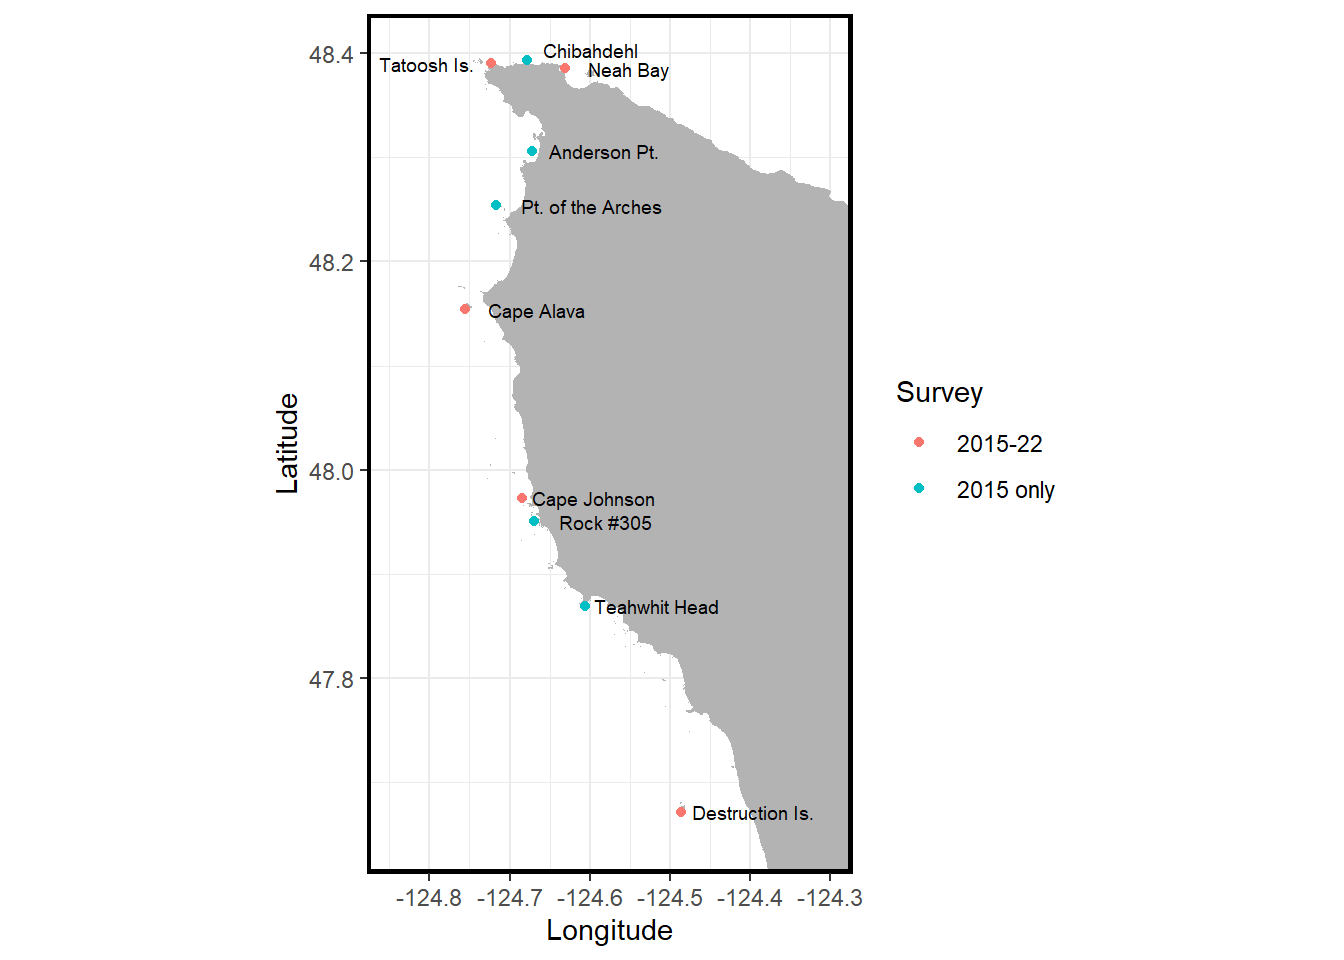
\includegraphics{~/Github/OCNMS/_01_Assessment-YOY-index//figures/fig-site-map-1.png}

}

\caption{\label{fig-site-map}Dive survey locations along the coast of
Washington state.}

\end{figure}

Transects were omitted from analyses if the horizontal visibility was
\textless2 m. The following tables (Table~\ref{tbl-samples-YS}) show how
the number fish transects with visibility \textgreater2 m were
distributed across depth, site, and years (Table~\ref{tbl-samples-YSD}),
as well as across sites and year (Table~\ref{tbl-samples-YS}). 2015
includes only surveys conducted at 5-m depth; other years have data
approximately evenly split between 5-m and 10-m depths.

\hypertarget{tbl-samples-YSD}{}
\begin{longtable}[]{@{}
  >{\raggedleft\arraybackslash}p{(\columnwidth - 14\tabcolsep) * \real{0.0602}}
  >{\raggedleft\arraybackslash}p{(\columnwidth - 14\tabcolsep) * \real{0.0602}}
  >{\raggedleft\arraybackslash}p{(\columnwidth - 14\tabcolsep) * \real{0.2289}}
  >{\raggedleft\arraybackslash}p{(\columnwidth - 14\tabcolsep) * \real{0.1566}}
  >{\raggedleft\arraybackslash}p{(\columnwidth - 14\tabcolsep) * \real{0.1325}}
  >{\raggedleft\arraybackslash}p{(\columnwidth - 14\tabcolsep) * \real{0.1807}}
  >{\raggedleft\arraybackslash}p{(\columnwidth - 14\tabcolsep) * \real{0.1084}}
  >{\raggedleft\arraybackslash}p{(\columnwidth - 14\tabcolsep) * \real{0.0723}}@{}}
\caption{\label{tbl-samples-YSD}Number of transects conducted by year,
site and depth zone. Only transects that had at least 2m visibility are
included}\tabularnewline
\toprule\noalign{}
\begin{minipage}[b]{\linewidth}\raggedleft
Year
\end{minipage} & \begin{minipage}[b]{\linewidth}\raggedleft
Zone
\end{minipage} & \begin{minipage}[b]{\linewidth}\raggedleft
Destruction Island
\end{minipage} & \begin{minipage}[b]{\linewidth}\raggedleft
Cape Johnson
\end{minipage} & \begin{minipage}[b]{\linewidth}\raggedleft
Cape Alava
\end{minipage} & \begin{minipage}[b]{\linewidth}\raggedleft
Tatoosh Island
\end{minipage} & \begin{minipage}[b]{\linewidth}\raggedleft
Neah Bay
\end{minipage} & \begin{minipage}[b]{\linewidth}\raggedleft
Total
\end{minipage} \\
\midrule\noalign{}
\endfirsthead
\toprule\noalign{}
\begin{minipage}[b]{\linewidth}\raggedleft
Year
\end{minipage} & \begin{minipage}[b]{\linewidth}\raggedleft
Zone
\end{minipage} & \begin{minipage}[b]{\linewidth}\raggedleft
Destruction Island
\end{minipage} & \begin{minipage}[b]{\linewidth}\raggedleft
Cape Johnson
\end{minipage} & \begin{minipage}[b]{\linewidth}\raggedleft
Cape Alava
\end{minipage} & \begin{minipage}[b]{\linewidth}\raggedleft
Tatoosh Island
\end{minipage} & \begin{minipage}[b]{\linewidth}\raggedleft
Neah Bay
\end{minipage} & \begin{minipage}[b]{\linewidth}\raggedleft
Total
\end{minipage} \\
\midrule\noalign{}
\endhead
\bottomrule\noalign{}
\endlastfoot
2016 & 5 & 0 & 4 & 6 & 4 & 4 & 18 \\
2016 & 10 & 3 & 6 & 6 & 4 & 6 & 25 \\
2017 & 5 & 3 & 5 & 4 & 3 & 4 & 19 \\
2017 & 10 & 0 & 4 & 6 & 4 & 4 & 18 \\
2018 & 5 & 0 & 4 & 4 & 8 & 4 & 20 \\
2018 & 10 & 0 & 3 & 8 & 7 & 8 & 26 \\
2019 & 5 & 4 & 4 & 8 & 8 & 7 & 31 \\
2019 & 10 & 8 & 7 & 8 & 6 & 8 & 37 \\
2021 & 5 & 4 & 8 & 7 & 8 & 8 & 35 \\
2021 & 10 & 3 & 8 & 7 & 6 & 8 & 32 \\
2022 & 5 & 0 & 0 & 4 & 8 & 8 & 20 \\
2022 & 10 & 0 & 0 & 7 & 6 & 5 & 18 \\
2023 & 5 & 6 & 8 & 8 & 8 & 10 & 40 \\
2023 & 10 & 4 & 9 & 8 & 8 & 7 & 36 \\
2024 & 5 & 0 & 0 & 4 & 4 & 4 & 12 \\
2024 & 10 & 3 & 0 & 3 & 9 & 9 & 24 \\
\end{longtable}

\newpage

\hypertarget{tbl-samples-YS}{}
\begin{longtable}[]{@{}lrrrrrrrr@{}}
\caption{\label{tbl-samples-YS}Number of transects conducted by year and
site. Only transects that had at least 2-m visibility are
included}\tabularnewline
\toprule\noalign{}
Site & 2016 & 2017 & 2018 & 2019 & 2021 & 2022 & 2023 & 2024 \\
\midrule\noalign{}
\endfirsthead
\toprule\noalign{}
Site & 2016 & 2017 & 2018 & 2019 & 2021 & 2022 & 2023 & 2024 \\
\midrule\noalign{}
\endhead
\bottomrule\noalign{}
\endlastfoot
Destruction Island & 3 & 3 & 0 & 12 & 7 & 0 & 10 & 3 \\
Cape Johnson & 10 & 9 & 7 & 11 & 16 & 0 & 17 & 0 \\
Cape Alava & 12 & 10 & 12 & 16 & 14 & 11 & 16 & 7 \\
Tatoosh Island & 8 & 7 & 15 & 14 & 14 & 14 & 16 & 13 \\
Neah Bay & 10 & 8 & 12 & 15 & 16 & 13 & 17 & 13 \\
TOTAL & 43 & 37 & 46 & 68 & 67 & 38 & 76 & 36 \\
\end{longtable}

\hypertarget{abundance-trends}{%
\section{Abundance trends}\label{abundance-trends}}

\hypertarget{recruitment-byt-young-of-year-abundance-trends}{%
\subsection{Recruitment: BYT young-of-year abundance
trends}\label{recruitment-byt-young-of-year-abundance-trends}}

To calculate the average density of BYT complex in each year, we first
calculate the mean density and standard error per site in each year.
This approach means we are treating each transect as a i.i.d. sample of
YOY density within each site and thus we ignore differences in abundance
by depth zone.

From these site-year level means, we calculated a year-specific mean
density by simulation. Specifically, for each year we independently drew
a mean density for each site using a t-distribution with \(\mu\) (the
estimated site mean), \(\sigma\) (the estimated site-specific standard
error) and degrees of freedom, \(\tau\). So for the \(i^{th}\)
realization, for site \(s\) in year \(y\) we have a predicted density,
\(X_{isy}\)

\begin{align}  & X_{isy} \sim T(\mu_{sy},\sigma_{sy},\tau_{sy}) \\ \end{align}

and then the predicted density for a single realization in a given year
is the mean among sites observed. We repeat the simulation 100,000 times
to provide an estimated mean density and uncertainty for a given year
(Fig.~\ref{fig-yoy-ts}).

Nearly all small rockfish fall into the 4 to 7 cm length range and all
are considered to have recruited from the plankton during the calender
year of the survey. Therefore, we view the density of \textless10cm
rockfish to be an indicator of recruitment for the black/yellowtail
rockfish complex (Fig.~\ref{fig-yoy-ts}).

\begin{figure}[H]

{\centering 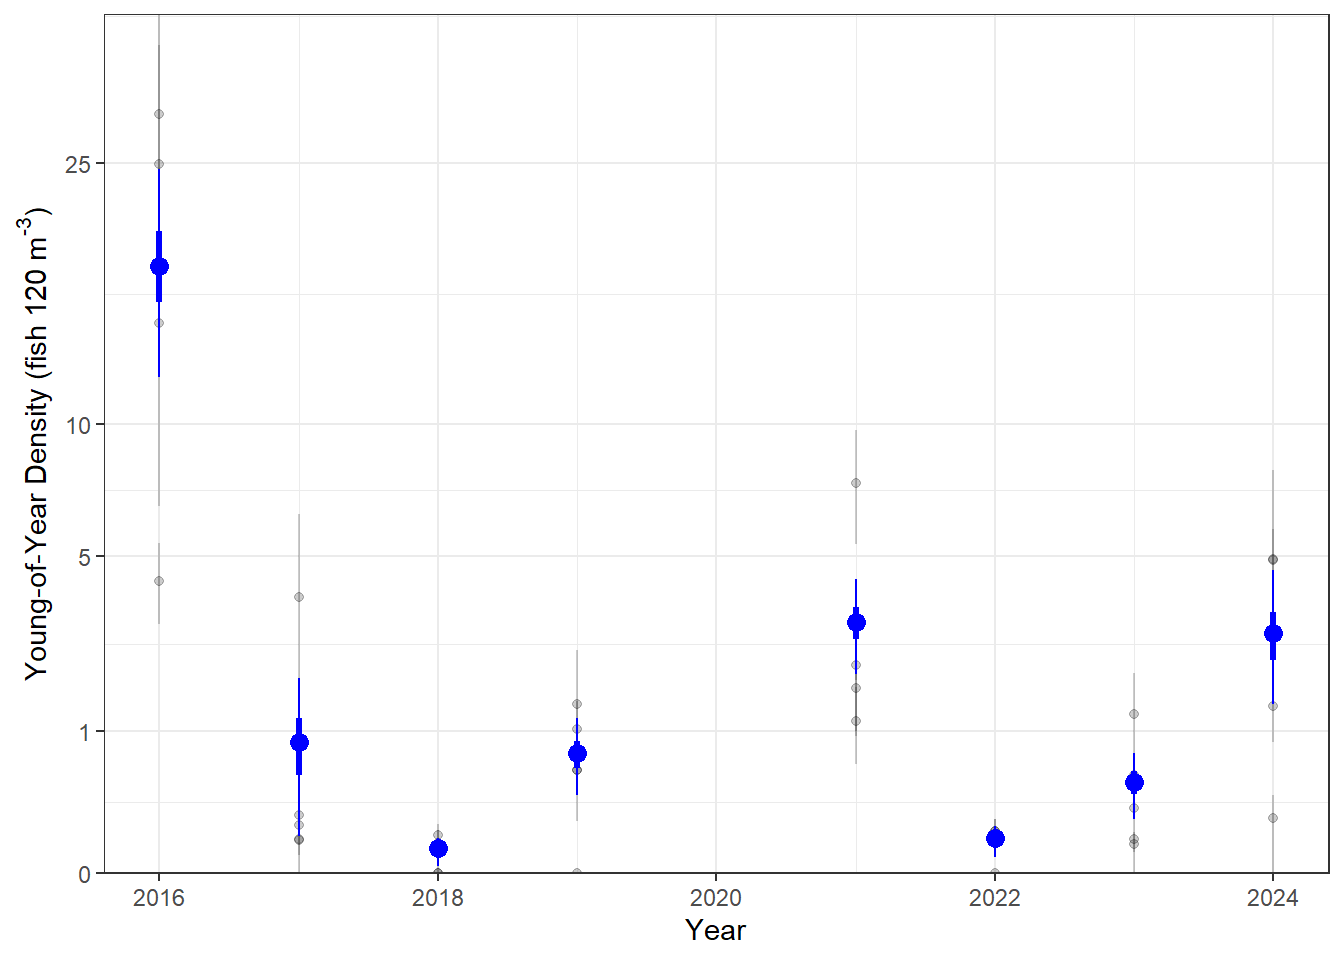
\includegraphics{~/Github/OCNMS/_01_Assessment-YOY-index//figures/fig-yoy-ts-1.png}

}

\caption{\label{fig-yoy-ts}Time-series of estimated young-of-year
rockfish (black-yellowtail complex) density on the Washington coast.
Black points show means and standard errors for individual sites. Blue
points show coastwide density estimates, interquartile range and 95\%
intervals for each year. Note y-axis is square root.}

\end{figure}

\newpage

\hypertarget{large-10-cm-total-length-black-rockfish}{%
\subsection{Large (\textgreater10 cm total length) black
rockfish}\label{large-10-cm-total-length-black-rockfish}}

We used the same approach as above to calculate the average density of
large black rockfish in each year (Fig.~\ref{fig-spp-ts}). Yellowtail
rockfish are not common in our dive surveys and are not considered
below.

\begin{figure}[H]

{\centering 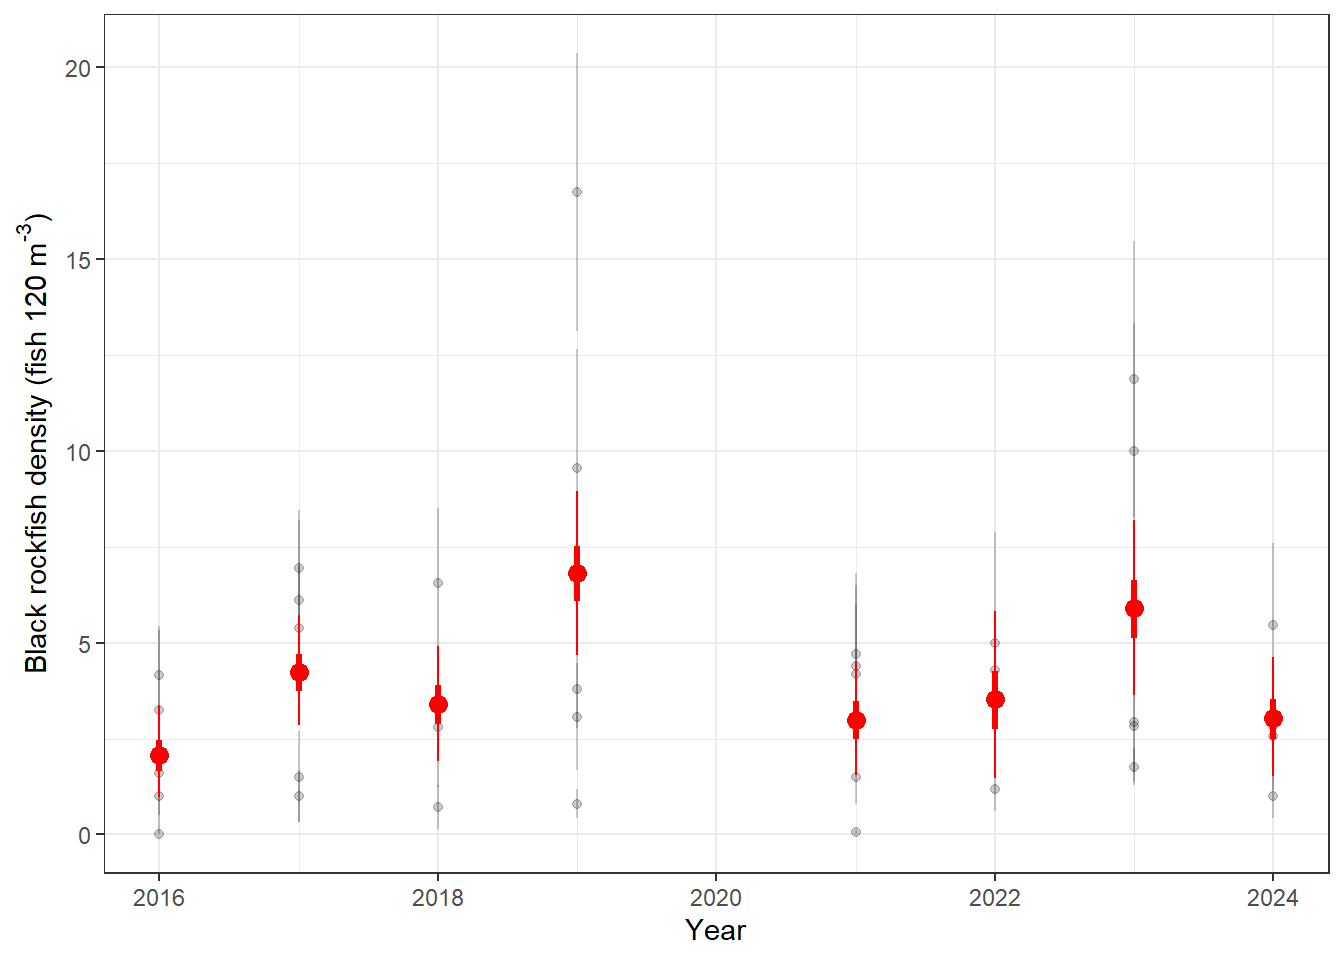
\includegraphics{~/Github/OCNMS/_01_Assessment-YOY-index//figures/fig-spp-ts-1.png}

}

\caption{\label{fig-spp-ts}Time-series of estimated black rockfish
density on the Washington coast. Black points show means and standard
errors for individual sites. Red points show coastwide density
estimates, interquartile range and 95\% intervals for each year}

\end{figure}

\newpage

\hypertarget{size-structure-of-black-rockfish-2015-2024}{%
\subsection{Size structure of black rockfish
2015-2024}\label{size-structure-of-black-rockfish-2015-2024}}

In addition to abundance data, we visually estimate size (total length)
for all individuals observed during the surveys. Young-of-year show
remarkably limited variation in size and so we exclude them from the
analysis. The data here are for black rockfish; yellowtail are not
presented because the adults are uncommon at our sites. Plots of size
distribution grouped into 5-cm bins are shown in
Figures~\ref{fig-spp-size-bin1} \& \ref{fig-size-bin2}.
Figure~\ref{fig-size-dist2} shows the size distribution 1-cm increments.

\begin{figure}[H]

{\centering 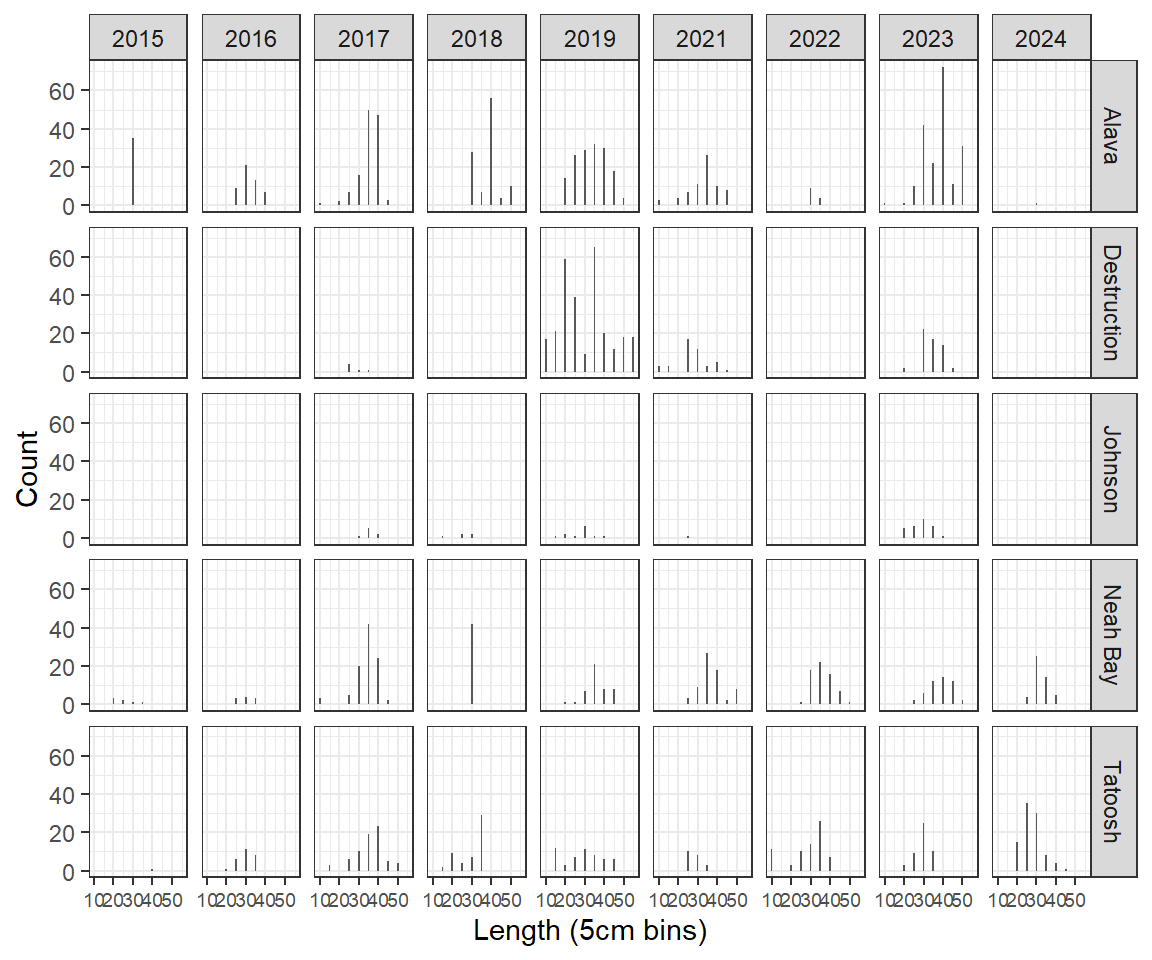
\includegraphics{~/Github/OCNMS/_01_Assessment-YOY-index//figures/fig-spp-size-bin1-1.png}

}

\caption{\label{fig-spp-size-bin1}Black rockcish size distributions by
5-cm size bins for years and sites.}

\end{figure}

\newpage

\begin{figure}[H]

{\centering 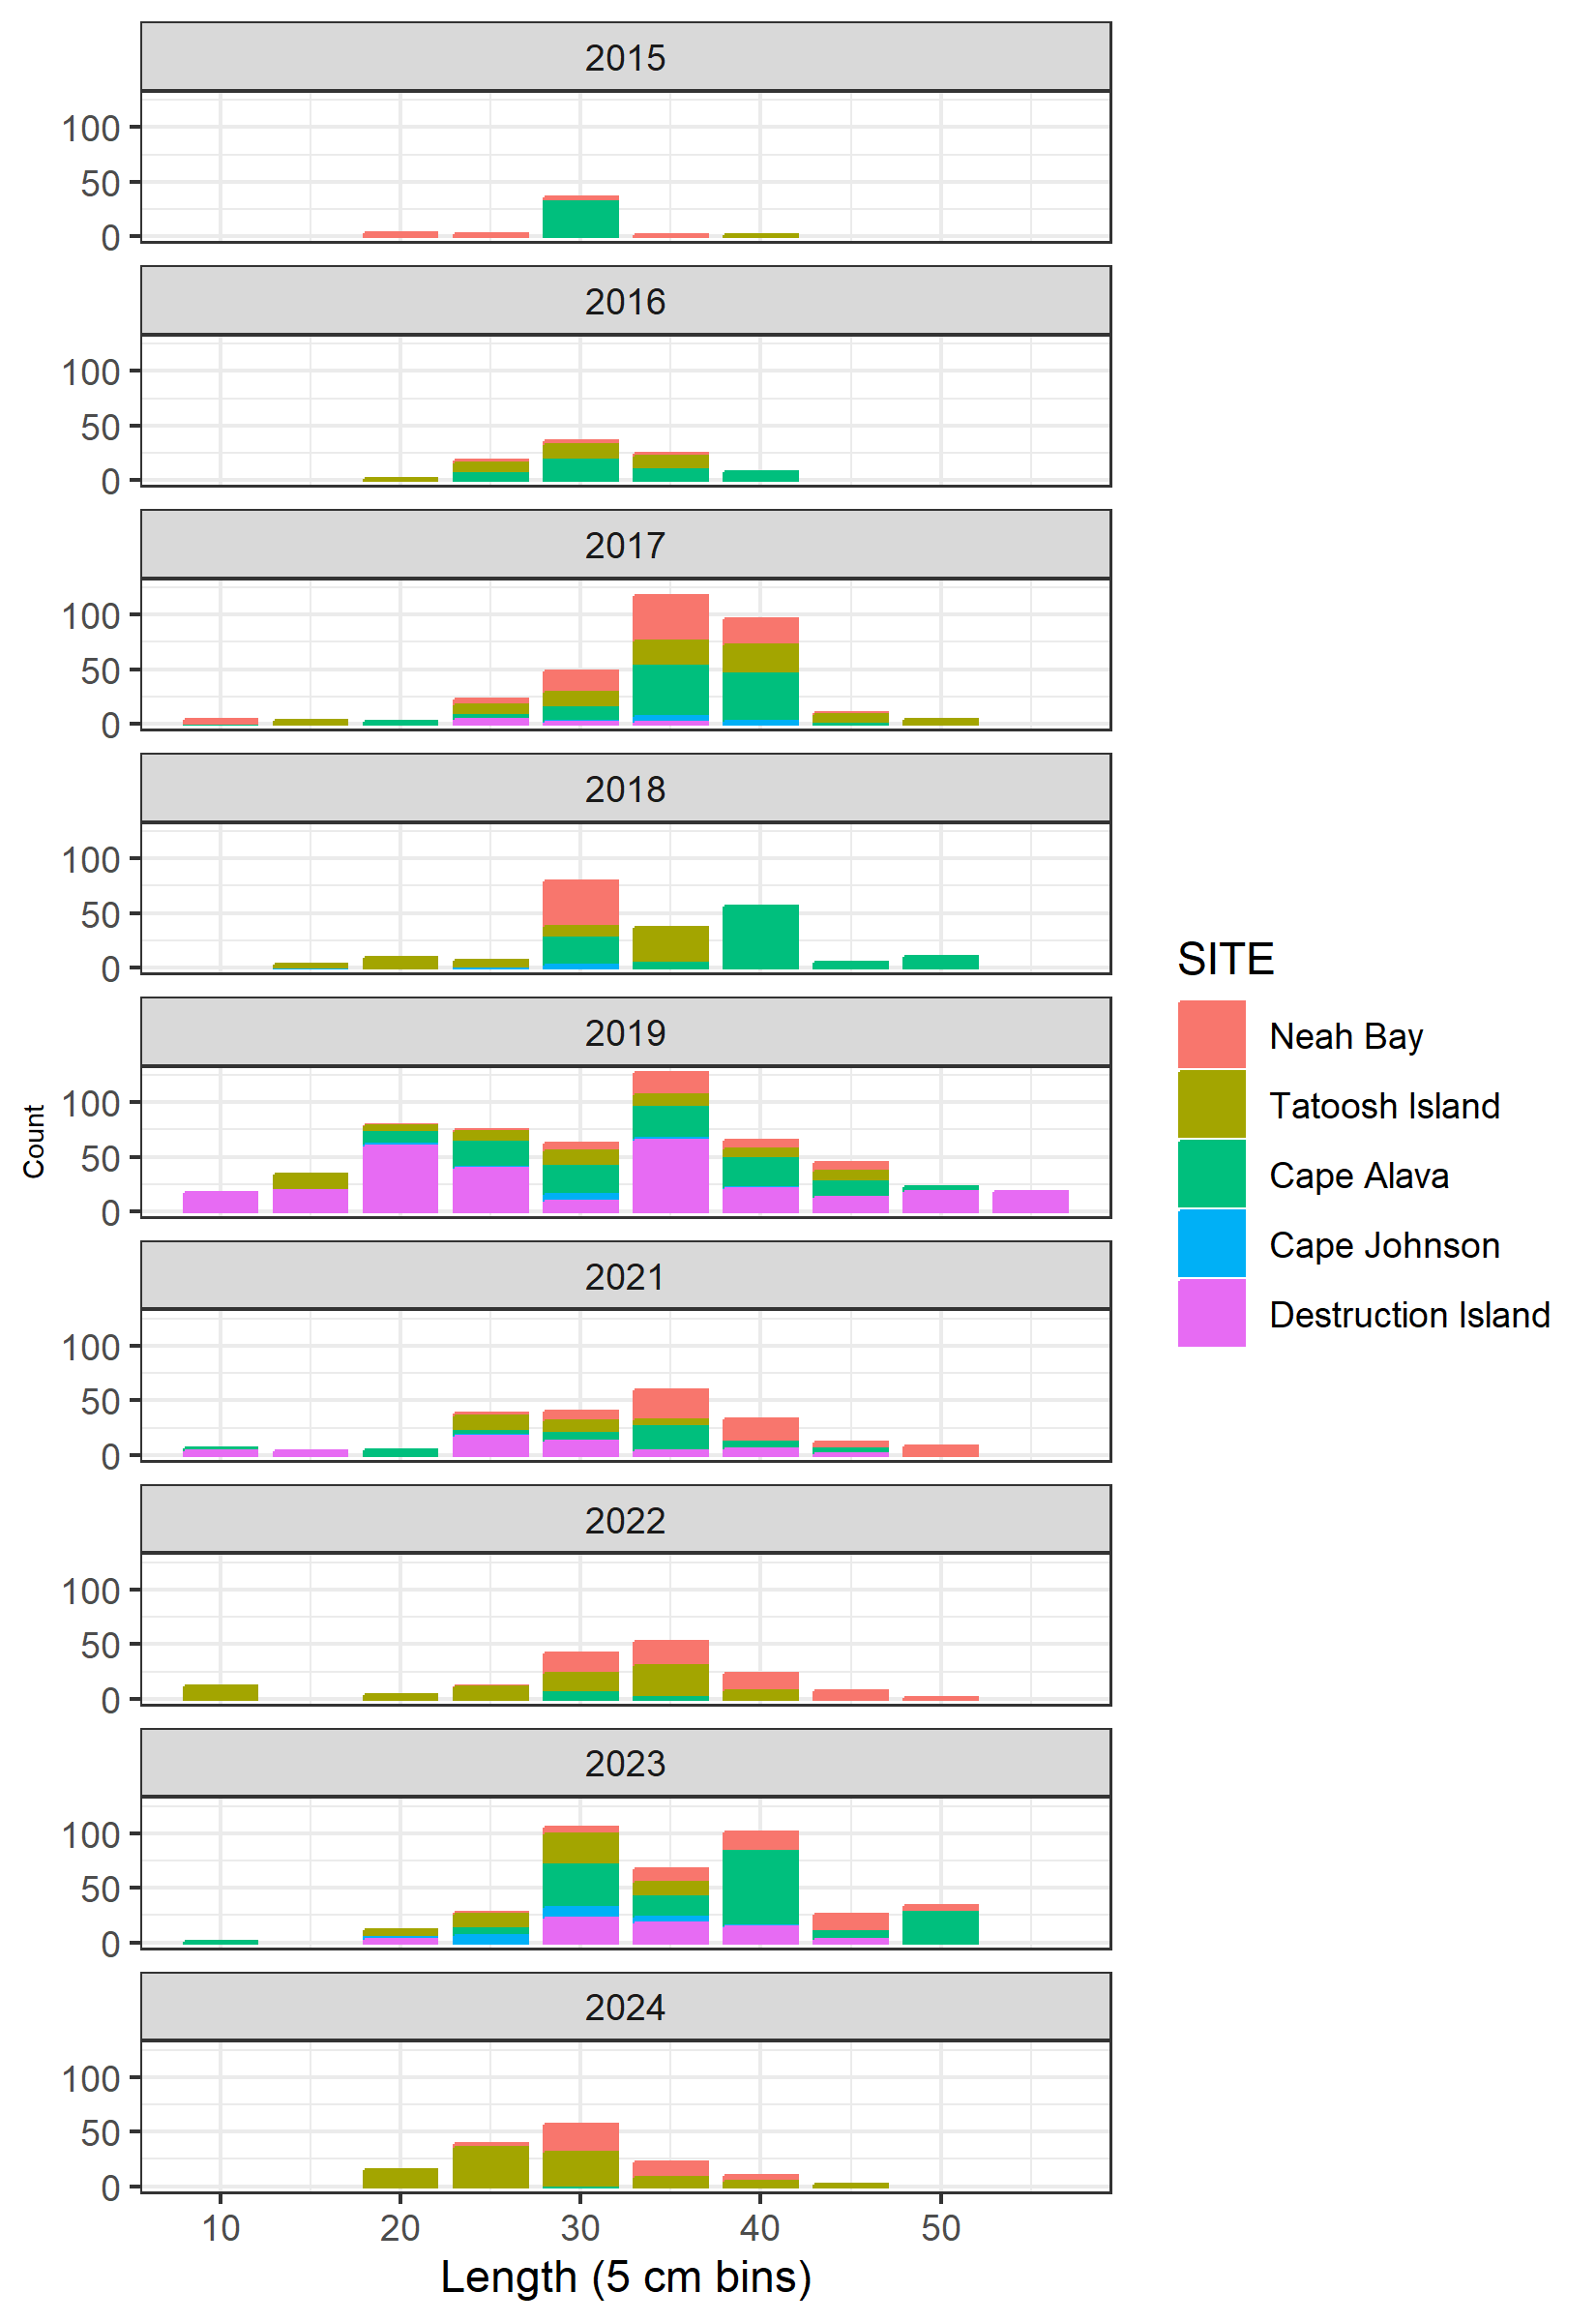
\includegraphics{~/Github/OCNMS/_01_Assessment-YOY-index//figures/fig-size-bin2-1.png}

}

\caption{\label{fig-size-bin2}Black rockfish size distribution by 5-cm
size bins plotted by site, summed across sites within each year}

\end{figure}

\newpage

\begin{figure}[H]

{\centering 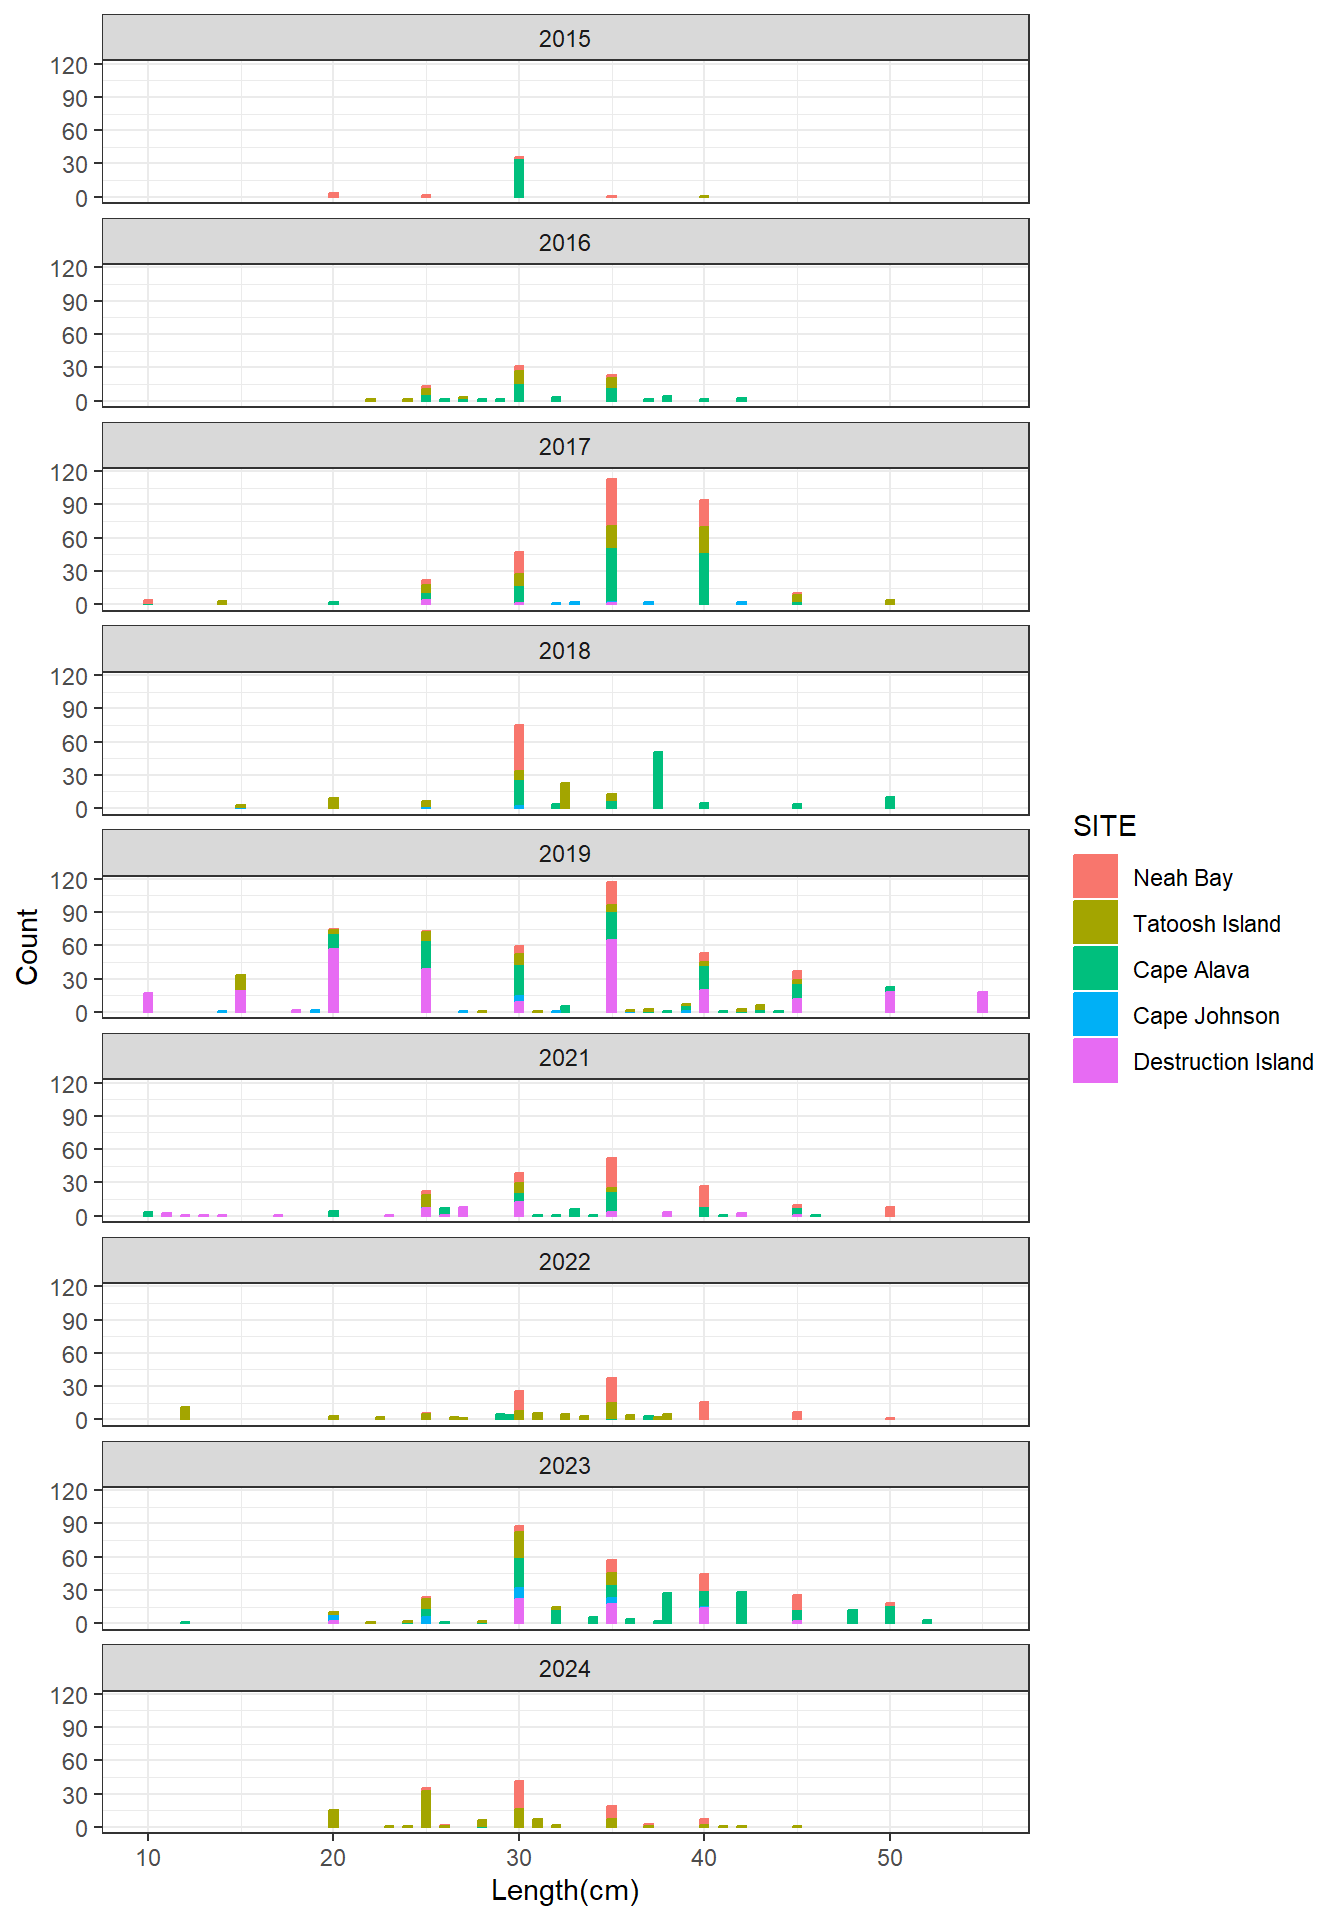
\includegraphics{~/Github/OCNMS/_01_Assessment-YOY-index//figures/fig-size-dist2-1.png}

}

\caption{\label{fig-size-dist2}Black rockfish size distribution by 1-cm
size bins plotted by site, summed across sites within each year.}

\end{figure}

\newpage

\hypertarget{references}{%
\section{References}\label{references}}

\hypertarget{refs}{}
\begin{CSLReferences}{1}{0}
\leavevmode\vadjust pre{\hypertarget{ref-johansson2018seasonal}{}}%
Johansson ML, Litz MN, Brodeur RD, et al (2018) {Seasonal distribution
of late larval and juvenile rockfish (\emph{Sebastes} spp.) and
associated environmental conditions off Oregon and Washington: new
insights based on genetics}. Fishery Bulletin 266--291

\leavevmode\vadjust pre{\hypertarget{ref-malone2022large}{}}%
Malone DP, Davis K, Lonhart SI, et al (2022) {Large-scale, multidecade
monitoring data from kelp forest ecosystems in California and Oregon
(USA)}

\leavevmode\vadjust pre{\hypertarget{ref-markel2020contrasting}{}}%
Markel RW, Shurin JB (2020) {Contrasting effects of coastal upwelling on
growth and recruitment of nearshore Pacific rockfishes (genus
\emph{Sebastes})}. Canadian Journal of Fisheries and Aquatic Sciences
77:950--962

\leavevmode\vadjust pre{\hypertarget{ref-shelton2018predictable}{}}%
Shelton AO, Harvey CJ, Samhouri JF, et al (2018) {From the predictable
to the unexpected: kelp forest and benthic invertebrate community
dynamics following decades of sea otter expansion}. Oecologia
188:1105--1119

\leavevmode\vadjust pre{\hypertarget{ref-tolimieri2023changes}{}}%
Tolimieri N, Shelton AO, Samhouri JF, et al (2023) {Changes in kelp
forest communities off Washington, USA, during and after the 2014-2016
marine heatwave and sea star wasting syndrome}. Marine Ecology Progress
Series 703:47--66

\end{CSLReferences}



\end{document}
